Wie bereits beschrieben, gehört der Bereich der Automatisierung zu den Grundpfeilern einer DevOps-Umgebung. 

Insbesondere aufgrund der immer größer werdenden Koplexität eingesetzter Technologien für den Softwareentwicklungs- und Deployment-Prozess, ist die Automatisierung im DevOps-Umfeld essentiell. 

Durch einen hohen Grad an Automatisierung sollen wiederholende Aufgaben reduziert werden, mit dem Ziel das Risiko manueller Fehler zu vermeiden und die Verschwendung von menschlichen Ressourcen zu minimieren.  

Gemäß des DevOps-Konzepts werden die Grundsätze des DevOps-Ansatzes durch den Aufbau einer Bereitstellungspipeline (engl. Deployment Pipeline) durchgesetzt.

Die Deployment-Pipeline besteht im Wesentlichen aus mehreren Continuous Integration und Continuous Delivery-Pipelines und kann als eine automatisierte Implementierung der Build-, Test-, Deployment- und Release-Prozesse einer Anwendung definiert werden. \cite{humble_why_2011}

Ziel des Continuous Deployments ist die vollständige Automatisierung des Deployments auf die Produktivumgebung und der Infrastruktur. 

Insbesondere die Testautomatisierung ist ein zentraler Bestandteil der Deployment Pipeline.

Jede neue Version des Codes wird über mehrere Schritte getestet, es werden Builds erstellt, wiederholt getestet und anschließend an die Produktivumgebung übergeben.

Im Hinblick auf eine ganzheitliche Automatisierung, ist es dem DevOps-Team möglich, alle Softwareversionen durch einen vollständig automatisierten Prozess bereitzustellen und freizugeben. 

Um die Rolle der Automatisierung voranzutreiben, werden möglichst viele vollautomatisierte Deployments auf die Produktivumgebung aufgesetzt. 

Während zu Beginn einfache Unit-Tests ausreichen, müssen mit fortschreitender Automatisierung zur Sicherstellung der Qualität Funktions-, Last- oder Integrationstests implementiert werden, bis ein manuelles Testen bestenfalls überflüssig wird. \cite[S. 27]{alt_innovationsorientiertes_2017}

Daher müssen die erfolgten Tests, bei steigender Automatisierung der Pipeline, so umfangreich wie möglich durchgeführt werden, um die Qualität und die Lauffähigkeit der Software sicherzustellen. \cite[S. 110 - 111]{wolff_continuous_2016}

Eine entsprechende Deployment-Pipeline kann durch den Einsatz passender Tools (dt. Werkzeuge)etabliert werden und stellt mit Hilfe miteinander kombinierter Tools eine optimale Abdeckung der Automatisierung sicher. \cite[S. 268]{tokarski_strategische_2018} 

Während anfänglich eine Toolchain für die Deployment-Pipeline ausreichend ist, muss diese mit steigender Verantwortung des DevOps-Teams für alle Bereiche erweitert werden. 

Werden die Deployments automatisch in die Produktivumgebung ausgeführt, sind die DevOps-Teams ab diesem Zeitpunkt in der Lage, jederzeit eine neue Funktion, Fehlerbehebung oder Anpassungen an der Infrastruktur, auszuliefern. \cite{juner_praxisbasierte_2017} 

\begin{figure}[h]
    \centering
    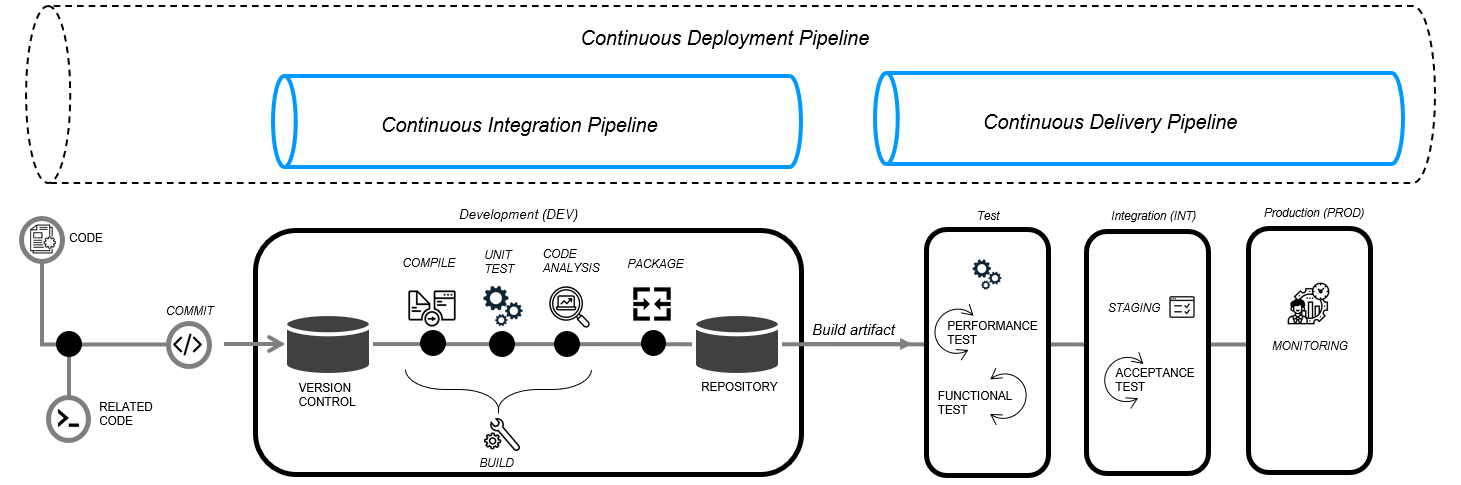
\includegraphics[scale=0.4]{Bilder/Continuous Deployment Pipeline.png}
    \caption{CI-Pipeline, angelehnt an \cite{balajee_what_2020}, \cite[S. 17]{sharma_devops_2017}}
\end{figure}

Mit der Deployment-Pipeline werden drei Ziele verfolgt. \cite[S. 3 - 4]{humble_continuous_2011} 

Zunächst ist jeder Schritt des Prozesses angefangen bei der Erstellung, des Einsatzes, des Testens und der Softwarefreigabe (End-to-End-Prozess) für alle sichtbar, wodurch die gesamte Zusammenarbeit gefördert wird. 

Mit jedem Schritt der erfolgreich durchlaufen ist, ist es wahrscheinlicher, dass die Kombination aus Code, Konfiguration, Umgebung und Daten einer neuen Version keine Fehler aufweist. 

Weiterhin wird das Feedback verbessert, indem die Probleme sehr zeitnah im Prozess erkannt und behoben werden können. 

Jede Deployment-Pipeline gestaltet sich oftmals von Projekt zu Projekt verschieden, je nachdem welche Anforderungen an die Software gefordert sind.  

In diesem Abschnitt werden sowohl die Integration als auch die Delivery Pipeline einzeln beschrieben und auf die Schritte näher eingegangen, die in einem Idealfall eintreten werden. 

\paragraph{Integration Pipeline} 

Continuous Integration wird zunächst bei jedem Einspielen von Code Commits automasiert angestoßen. \cite[S. 266]{tokarski_strategische_2018}. 

In diesem Zuge wird der Code kompiliert und idealerweise alle Unit-Tests durchgeführt.  

Unit-Tests ermöglichen ein schnelles Testen des Verhaltens von kleinen Codeänderungen isoliert von den anderen Komponenten der Software. \cite[S. 60]{humble_continuous_2011} 

Die Unit-Tests erfolgen automatisiert, wodurch die Entwickler sicherstellen können, dass die vorgenommenen Änderungen tatsächlich funktionieren und das ein kontinuierliches Deployment kleiner Inkremente auf die Integrationsumgebung möglich ist.

Nachdem das Testen erfolgreich abgeschlossen wurde, wird der Commit angenommen und die statische Analyse des Quellcodes kann beginnen. \cite[S. 61]{verona_practical_2016} 

Diese Analyse liefert Informationen über den Zustand des Codes, über Defekte, Design-Probleme oder ob Schwachstellen in den Bibliotheken von Drittanbietern gefunden wurden. \cite[S. 61]{verona_practical_2016} 

Nach der Validierung des Quellcodes wird dieser als ein Build in einem Repository veröffentlicht.

Für den Schritt des Erstellen des Builds und das Testen ist der Integrationsserver (CI-Server) zuständig. 

Bei Änderungen des Builds werden erneut Unit-Tests durchgeführt, um die Funktionalität der Anpassung sicherzustellen. \cite[S. 57]{forsgren_mindset_2019} 

Wichtige Voraussetzung für die Integration der CI-Pipeline ist zunächst die Verwendung einer Versionskontrolle. \cite[S. 100 - 101]{bass_devops_2015}, \cite[S. 57]{forsgren_mindset_2019} 

Die verteilte Versionskontrolle ermöglicht es einzelnen Entwickelern, unabhängig von ihrem Standort oder von der Funktion, an der sie arbeiten, parallel zusammenzuarbeiten.

Aufgrund der sofortigen Erfassung kleiner Änderungen mittels der Versionskontrolle, können Anwendungen die fehlerhaft schnell gefunden und sofort beseitigt werden. \cite[S. 57]{humble_continuous_2011}

Um automatische Tests und Zusammenspiel aller Funktionen auf dem integrierten Master-Branch sicherzustellen und zeitaufwendige Code-Merges zu vermeiden, müssen insbesondere Feature-Branches bei der Entwicklung kurz gehalten werden. \cite{meyer_continuous_2014}

Die Grundidee des Workflows mittels Feature-Branch besteht darin, dass die gesamte Entwicklung der Features in einem Branch in der Versionskontrolle und nicht auf dem Master-Branch stattfindet. \cite[S. 44 - 45]{verona_practical_2016} 

Entwickler können eingegrenzt an einem bestimmten Feature arbeiten, ohne die Codebasis innerhalb des Master-Branches zu behindern.  

Sobald Änderungen mit dem Main-Branch zusammengeführt werden, werden diese in automatischen Build-Prozessen und mittels Tests validiert. 

Sollte eine Rückführung des neuen Codes aus den sich verändernden Main-Branch stattfinden, so führt langwieriges Branchen zu einem großen Aufwand. \cite{juner_praxisbasierte_2017}  

\paragraph{Delivery Pipeline} 

Continuous Delivery erweitert die CI-Pipeline, um die erfolgreich durchgeführten Builds automatisch in produktionsähnlichen Testumgebungen bereitszustellen, in denen funktionale Test, Integrationstests und Performance-Tests durchgeführt werden. \cite[S. 17]{sharma_devops_2017}

Auslöser für die CD-Pipeline ist jedes neue Build-Artefakt, welches im Repository veröffentlicht wird.

Zusätzlich zum Quellcode werden alle Build-Artefakte innerhalb des Repositorys gespeichert, während die gleichen Versionen für die Entwicklungs-, Test- sowie Produktionsumgebung verwendet werden. \cite[S. 109 - 110]{kim_devops-handbuch_2017}

Im nächsten Schritt wird der Code zusammen mit der entsprechenden Konfiguration in eine ausführbare Anwendung gebaut. 

Das Ergebnis ist der Artefakt Build, der ab diesem Zeitpunkt nicht mehr verändert werden sollte. 

In diesem Rahmen führt der CI-Server systemübergreifende Integrationstests an dem jeweiligen Build auf der Integrationsumgebung vor, um die fehlerfreie Interaktion der gesamten Komponenten miteinander zu testen. \cite[S. 122]{kim_devops-handbuch_2017} 

Während der Integrationstest wird eine Anbindung zu einer Testdatenbank konfiguriert, die aus einer ausreichenden Menge von Daten besteht, um die mit der Integration verbundenen automatisierten Tests durchzuführen. \cite[S. 100 - 101]{bass_devops_2015}

Als nächsten Schritt wird die Software innerhalb der Staging-Umgebung testweise betrieben, ohne die Interaktion der produktiv betriebenen Services. 

Die Konfiguration der Anwendung sollte innerhalb dieser Phase den vorläufigen Produktionszustand aufweisen. \cite[S. 100 - 101]{bass_devops_2015} 

Anschließend erfolgen die Akzeptanztests, die mit einer Anzahl von Nutzern erfolgen. 

Diese testen die Anwendung mittels festgelegter Testfälle oder verwenden diese wie vorgesehen und können dadurch dem DevOps-Team direkten Feedback über Schwachstellen oder funktionale Probleme liefern. \cite[S. 16 - 18]{sharma_devops_2017}

Ferner können die Akzeptanztests auch automatisiert eingesetzt werden, was wiederrum den Grad der Wiederholbarkeit erhöht. 

Im Anschluss werden nicht-funktionale Tests und Performance-Tests durchgeführt.

Im besten Fall wird der Build durch die CD-Pipeline automatisch in die Produktivumgebung bereitgestellt, vorausgesetzt alle Tests wurden erfolgreich bestanden, anderenfalls wird das Deployment gestoppt und das Team wird über den Zustand des Builds informiert. \cite[S. 64]{forsgren_mindset_2019} 

Nachdem die Anwendung auf den normalen Produktivumgebung bereitgestellt wird, läuft diese konstant in einer Version oder aus einer Kombination von mehreren Versionen (Microservices). \cite[S. 86]{kim_devops-handbuch_2017}  

Die Architektur des Microservices bildet die Grundlage für den DevOps-Ansatz und beschreibt den Aufbau von Anwendungen, basierend auf eine große Anzahl an kleinen Services. \cite{sollner_devops_2017}

Diese Services bestehen aus kleinen separaten funktionalen Codeteilen, die miteinander interagieren und miteinander ein Anwendungssystem abbilden.  

Oftmals wird nur eine Funktionalität abgebildet und kommuniziert mit anderen Services über eine definierte Schnittstelle. 

Mittels Microservices lassen sich einzelne Funktionalitäten leicht und schnell deployen und anpassen, wodurch das gesamte Deployment erhöht, die Wartung vereinfacht und das restliche System nicht gefährdet wird. \cite[S. 85 - 86]{kim_devops-handbuch_2017}  

Dieser Ansatz vereinfacht die Methode des Continuous Integration. \\

Insgesamt lässt sich Continuous Deployment als einen automatischen, regelmäßigen Prozess der Bereitstellung erfolgreicher Builds in die Produktivumgebung beschreiben.

Allerdings ist, \textit{die Fähigkeit zur kontinuierlichen Bereitstellung wichtiger als die tatsächliche kontinuierliche Bereitstellung für die Produktion}. \cite[S. 19]{sharma_devops_2017}

Damit schlussfolgert Sharma, dass Continuous Delivery ein Muss ist, aber Continuous Deployment als eine Option angesehen werden kann.  

%Frage an Daniel: 
%1. Feature-Toggling, verschiedenes Testing (A/B-Tests, Canary-Tests, Live Test oder Beta-Tests), oder das Blue/Green Deployment erwähnen/beschreiben/erklären?????
%2. Irgeendwie bin ich mir nicht sicher, bei der Kapitelüberschrift---> Idee?





 











  











 





